\documentclass[../../FisicaTeorica.tex]{subfiles}

\begin{document}
\begin{comment}
\section{Riepilogo}
\textbf{Evoluzione temporale}: se non osserviamo l'evoluzione degli 
stati è data da $U(t)\ket{\psi}U(t)=e^{-\frac{i}{\hbar}tH}$, mentre quella delle osservabili è $A^H(t)=U^\dag(t)AU(t)$, e in entrambi i casi si tratta di una evoluzione deterministica.\\
Se invece eseguiamo un'osservazione sul sistema, allora vale il postulato di proiezione di Von Neumann, per cui se una misura ideale di prima specie di $A$ in $\ket{\psi}$ dà risultato in $\Delta \subseteq \bb{R}$, dopo la misura lo stato è descritto da:
$$
P^A(\Delta)\ket{\psi}\equiv \sum_{\lambda_n\in \sigma_P(A)\subseteq \Delta}\sum_{r=1}^{d(\lambda_n)}\ket{\lambda_n,r}\braket{\lambda_n,r|\psi}+
\int_{\sigma_C(A)\cap\Delta}d\lambda\,\sum_{r=1}^{d(\lambda)}\ket{\lambda,r}\braket{\lambda,r|\psi}
$$
In particolare il \textit{risultato} di una misura ideale di prima specie è \textit{univoco}, mentre quello di una misura ideale è uno qualsiasi tra quelli compatibili con la misura in $\Delta$.\\

\section{Nuova lezione}
\end{comment}
\subsection{Differenze tra \MC e \MQ} 
\lesson{16}{5/11/2018}
Nonostante l'apparenza\marginpar{Differenze qualitative}, la proiezione di von Neumann è ben diversa dalla \q{proiezione} di uno stato misto classico generata da una misura che riduce  l'indeterminazione di un'osservabile, aumentando l'informazione disponibile allo sperimentatore.\\
Per esempio, consideriamo un sistema \q{classico}, in cui una \textit{formica} è lasciata libera di spostarsi all'interno di una stanza. Prima di un'osservazione non sappiamo esattamente in che punto si trovi - possiamo al più costruire una \textit{distribuzione di probabilità} per la sua posizione. Per esempio, se la formica è partita al centro della stanza, dato che si muove lentamente, dopo un minuto sarà probabilmente ancora nei pressi del centro.\\
Se ora entriamo nella stanza e osserviamo una certa regione $A$ (compiendo così una misura) avremo una certa probabilità di trovare o meno la formica in $A$.\\
Se la troviamo lì, immediatamente la distribuzione di probabilità \q{collassa} su $A$ - dato che siamo certi che la posizione della formica a quell'istante è in $A$.\\
Allo stesso modo, se non avessimo trovato la formica in $A$, immediatamente la densità di probabilità in $A$ si annullerebbe, poiché sapremmo con certezza che la formica non è in $A$.\\
Tutto ciò sembra ovvio e banale, e non crea problemi poiché abbiamo fatto uso di una distribuzione di probabilità in primo luogo a seguito di una nostra ignoranza - si tratta di un \textit{artifizio} matematico che non ha alcun significato fisico: il sistema si evolve \textit{classicamente} indipendentemente dalle misure che facciamo, e in particolare indipendentemente da come \textit{evolve} a seguito delle misure la distribuzione di probabilità. In effetti, il sistema prima della misura è in uno \textbf{stato misto}: abbiamo tante possibilità per la posizione della formica, ciascuna \textit{pesata} dalla sua probabilità. Dopo la misura, se sappiamo la posizione della formica, l'informazione sulla formica si è accresciuta. Nel caso limite in cui conosciamo sia posizione che momento della formica, lo stato del sistema sarà addirittura puro: l'unica differenza sta perciò nello sperimentatore, che dopo la misura ha più informazioni sul sistema.\\
In \MQ, invece, l'evoluzione del sistema comporta l'evoluzione della sua distribuzione di probabilità - che emerge anche per \textbf{stati puri}. In effetti, se consideriamo l'analogo problema di una particella a energia fissata in una buca unidimensionale infinita, abbiamo a che fare con un sistema descritto da uno stato puro, e dopo la misura (ideale di prima specie) si ottiene ancora uno stato puro, diverso dal primo. Non abbiamo quindi \textit{acquisito informazione e basta}, ma \textit{diminuito} l'incertezza su alcune osservabili a discapito di altre, mantenendo comunque la stessa \q{quantità} (massimale) di informazione. Il sistema dopo la misura, tuttavia, si comporterà in modo diverso da quello prima: l'atto di misura \textit{ha perturbato} l'evoluzione del sistema.\\

Rendiamo più concreto (matematicamente) tale esempio.\\
Consideriamo \textit{classicamente}\marginpar{Esempio numerico: misura in \MC} una particella libera di muoversi lungo una dimensione, di cui supponiamo conoscere l'impulso $p_0$ classico, e di sapere che la sua posizione ha una distribuzione di probabilità $\rho(x)$.\\
%Disegno di una distribuzione gaussiana \rho(x), con evidenziato un intervallino \Delta [IMMAGINE]
A $t=0$ eseguiamo una \q{misura ideale di prima specie} nel senso sopra descritto, ma a livello classico, volta a verificare se la particella è in $\Delta$.\\
Se la misura trova la particella in $\Delta$, lo stato del sistema appena dopo (a $t=0^+$) sarà dato dalla \textit{proiezione}:
\[
f(x,p)_{t=0} = \rho(x)\delta(p-p_0)\to 
f(x,p)_{t=0^+} =
\frac{\rho(x)\chi_\Delta(x)\delta(p-p_0)}{\displaystyle \int_\Delta \rho(x)\,dx}
\]
per cui a $t=0^+$ la distribuzione di probabilità è annullata al di fuori di $\Delta$ dalla funzione caratteristica $\chi_\Delta$, mentre per $x\in \Delta$ ha lo stesso andamento di prima (a meno del fattore di normalizzazione dato dal denominatore).\\
Notiamo allora che l'indeterminazione in $x$ è diminuita \textbf{senza modificare} quella in $p$, cioè e la \q{fisica del sistema non è cambiata} (ossia il suo comportamento) con l'acquisizione di informazione.\\

Nel caso quantistico\marginpar{Esempio numerico: misura in \MQ}, invece, sia $\ket{\psi}$ che la sua proiezione di von Neumann $P^X(\Delta)\ket{\psi}$ sono entrambi \textbf{stati puri}, e quindi di conoscenza \textbf{massimale}, pertanto il miglioramento della conoscenza di $X$ deve comportare il peggioramento della conoscenza di altre osservabili (sicuramente $\ket{\psi}\bra{\psi}$, dato che non sappiamo più se la particella sia nello stato $\ket{\psi}$ - e anzi, nel caso di una misura ideale proprio non ci sta - e probabilmente anche di $p$ per il principio di indeterminazione).\\
Diversamente dal caso classico abbiamo perciò modificato la \q{fisica} (il comportamento) del sistema.\\

\begin{center}
\tikzset{every picture/.style={line width=0.75pt}} %set default line width to 0.75pt        

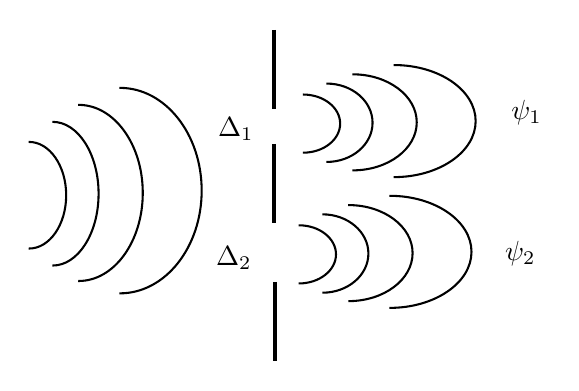
\begin{tikzpicture}[x=0.75pt,y=0.75pt,yscale=-1,xscale=1]
%uncomment if require: \path (0,382); %set diagram left start at 0, and has height of 382

%Straight Lines [id:da10084162796365637] 
\draw [line width=1.5]    (196.5,97) -- (196.5,135) ;


%Straight Lines [id:da7924850248248765] 
\draw [line width=1.5]    (196.5,152) -- (196.5,190) ;


%Straight Lines [id:da11357677903705787] 
\draw [line width=1.5]    (197,218.5) -- (197,256.5) ;


%Shape: Arc [id:dp7657989221858108] 
\draw  [draw opacity=0][line width=0.75]  (208.26,219.23) .. controls (208.29,219.23) and (208.33,219.23) .. (208.36,219.23) .. controls (218.22,219.23) and (226.22,212.95) .. (226.22,205.22) .. controls (226.22,197.48) and (218.22,191.21) .. (208.36,191.21) .. controls (208.32,191.21) and (208.29,191.21) .. (208.25,191.21) -- (208.36,205.22) -- cycle ; \draw  [line width=0.75]  (208.26,219.23) .. controls (208.29,219.23) and (208.33,219.23) .. (208.36,219.23) .. controls (218.22,219.23) and (226.22,212.95) .. (226.22,205.22) .. controls (226.22,197.48) and (218.22,191.21) .. (208.36,191.21) .. controls (208.32,191.21) and (208.29,191.21) .. (208.25,191.21) ;
%Shape: Arc [id:dp3319913384117632] 
\draw  [draw opacity=0][line width=0.75]  (219.61,223.69) .. controls (219.65,223.69) and (219.68,223.69) .. (219.71,223.69) .. controls (231.93,223.69) and (241.83,215.24) .. (241.83,204.81) .. controls (241.83,194.39) and (231.93,185.93) .. (219.71,185.93) .. controls (219.68,185.93) and (219.64,185.93) .. (219.61,185.93) -- (219.71,204.81) -- cycle ; \draw  [line width=0.75]  (219.61,223.69) .. controls (219.65,223.69) and (219.68,223.69) .. (219.71,223.69) .. controls (231.93,223.69) and (241.83,215.24) .. (241.83,204.81) .. controls (241.83,194.39) and (231.93,185.93) .. (219.71,185.93) .. controls (219.68,185.93) and (219.64,185.93) .. (219.61,185.93) ;
%Shape: Arc [id:dp9446365968081196] 
\draw  [draw opacity=0][line width=0.75]  (232.13,227.75) .. controls (232.17,227.75) and (232.21,227.75) .. (232.25,227.75) .. controls (249.3,227.75) and (263.12,217.39) .. (263.12,204.61) .. controls (263.12,191.83) and (249.3,181.47) .. (232.25,181.47) .. controls (232.21,181.47) and (232.16,181.47) .. (232.12,181.47) -- (232.25,204.61) -- cycle ; \draw  [line width=0.75]  (232.13,227.75) .. controls (232.17,227.75) and (232.21,227.75) .. (232.25,227.75) .. controls (249.3,227.75) and (263.12,217.39) .. (263.12,204.61) .. controls (263.12,191.83) and (249.3,181.47) .. (232.25,181.47) .. controls (232.21,181.47) and (232.16,181.47) .. (232.12,181.47) ;
%Shape: Arc [id:dp9971731130514143] 
\draw  [draw opacity=0][line width=0.75]  (251.98,231) .. controls (252.02,231) and (252.07,231) .. (252.12,231) .. controls (273.87,231) and (291.5,218.91) .. (291.5,204) .. controls (291.5,189.09) and (273.87,177) .. (252.12,177) .. controls (252.07,177) and (252.02,177) .. (251.97,177) -- (252.12,204) -- cycle ; \draw  [line width=0.75]  (251.98,231) .. controls (252.02,231) and (252.07,231) .. (252.12,231) .. controls (273.87,231) and (291.5,218.91) .. (291.5,204) .. controls (291.5,189.09) and (273.87,177) .. (252.12,177) .. controls (252.07,177) and (252.02,177) .. (251.97,177) ;
%Shape: Arc [id:dp7946417109385449] 
\draw  [draw opacity=0][line width=0.75]  (210.26,156.23) .. controls (210.29,156.23) and (210.33,156.23) .. (210.36,156.23) .. controls (220.22,156.23) and (228.22,149.95) .. (228.22,142.22) .. controls (228.22,134.48) and (220.22,128.21) .. (210.36,128.21) .. controls (210.32,128.21) and (210.29,128.21) .. (210.25,128.21) -- (210.36,142.22) -- cycle ; \draw  [line width=0.75]  (210.26,156.23) .. controls (210.29,156.23) and (210.33,156.23) .. (210.36,156.23) .. controls (220.22,156.23) and (228.22,149.95) .. (228.22,142.22) .. controls (228.22,134.48) and (220.22,128.21) .. (210.36,128.21) .. controls (210.32,128.21) and (210.29,128.21) .. (210.25,128.21) ;
%Shape: Arc [id:dp23616376305437914] 
\draw  [draw opacity=0][line width=0.75]  (221.61,160.69) .. controls (221.65,160.69) and (221.68,160.69) .. (221.71,160.69) .. controls (233.93,160.69) and (243.83,152.24) .. (243.83,141.81) .. controls (243.83,131.39) and (233.93,122.93) .. (221.71,122.93) .. controls (221.68,122.93) and (221.64,122.93) .. (221.61,122.93) -- (221.71,141.81) -- cycle ; \draw  [line width=0.75]  (221.61,160.69) .. controls (221.65,160.69) and (221.68,160.69) .. (221.71,160.69) .. controls (233.93,160.69) and (243.83,152.24) .. (243.83,141.81) .. controls (243.83,131.39) and (233.93,122.93) .. (221.71,122.93) .. controls (221.68,122.93) and (221.64,122.93) .. (221.61,122.93) ;
%Shape: Arc [id:dp4194359729685173] 
\draw  [draw opacity=0][line width=0.75]  (234.13,164.75) .. controls (234.17,164.75) and (234.21,164.75) .. (234.25,164.75) .. controls (251.3,164.75) and (265.12,154.39) .. (265.12,141.61) .. controls (265.12,128.83) and (251.3,118.47) .. (234.25,118.47) .. controls (234.21,118.47) and (234.16,118.47) .. (234.12,118.47) -- (234.25,141.61) -- cycle ; \draw  [line width=0.75]  (234.13,164.75) .. controls (234.17,164.75) and (234.21,164.75) .. (234.25,164.75) .. controls (251.3,164.75) and (265.12,154.39) .. (265.12,141.61) .. controls (265.12,128.83) and (251.3,118.47) .. (234.25,118.47) .. controls (234.21,118.47) and (234.16,118.47) .. (234.12,118.47) ;
%Shape: Arc [id:dp16466168017569305] 
\draw  [draw opacity=0][line width=0.75]  (253.98,168) .. controls (254.02,168) and (254.07,168) .. (254.12,168) .. controls (275.87,168) and (293.5,155.91) .. (293.5,141) .. controls (293.5,126.09) and (275.87,114) .. (254.12,114) .. controls (254.07,114) and (254.02,114) .. (253.97,114) -- (254.12,141) -- cycle ; \draw  [line width=0.75]  (253.98,168) .. controls (254.02,168) and (254.07,168) .. (254.12,168) .. controls (275.87,168) and (293.5,155.91) .. (293.5,141) .. controls (293.5,126.09) and (275.87,114) .. (254.12,114) .. controls (254.07,114) and (254.02,114) .. (253.97,114) ;
%Shape: Arc [id:dp19423318963830627] 
\draw  [draw opacity=0][line width=0.75]  (78.18,202.41) .. controls (78.24,202.41) and (78.3,202.41) .. (78.36,202.41) .. controls (88.22,202.41) and (96.22,190.92) .. (96.22,176.73) .. controls (96.22,162.55) and (88.22,151.05) .. (78.36,151.05) .. controls (78.29,151.05) and (78.23,151.05) .. (78.17,151.05) -- (78.36,176.73) -- cycle ; \draw  [line width=0.75]  (78.18,202.41) .. controls (78.24,202.41) and (78.3,202.41) .. (78.36,202.41) .. controls (88.22,202.41) and (96.22,190.92) .. (96.22,176.73) .. controls (96.22,162.55) and (88.22,151.05) .. (78.36,151.05) .. controls (78.29,151.05) and (78.23,151.05) .. (78.17,151.05) ;
%Shape: Arc [id:dp7301501317551493] 
\draw  [draw opacity=0][line width=0.75]  (89.53,210.6) .. controls (89.59,210.6) and (89.65,210.6) .. (89.71,210.6) .. controls (101.93,210.6) and (111.83,195.1) .. (111.83,175.99) .. controls (111.83,156.87) and (101.93,141.38) .. (89.71,141.38) .. controls (89.65,141.38) and (89.59,141.38) .. (89.52,141.38) -- (89.71,175.99) -- cycle ; \draw  [line width=0.75]  (89.53,210.6) .. controls (89.59,210.6) and (89.65,210.6) .. (89.71,210.6) .. controls (101.93,210.6) and (111.83,195.1) .. (111.83,175.99) .. controls (111.83,156.87) and (101.93,141.38) .. (89.71,141.38) .. controls (89.65,141.38) and (89.59,141.38) .. (89.52,141.38) ;
%Shape: Arc [id:dp24497387472419674] 
\draw  [draw opacity=0][line width=0.75]  (102.03,218.04) .. controls (102.1,218.04) and (102.17,218.05) .. (102.25,218.05) .. controls (119.3,218.05) and (133.12,199.05) .. (133.12,175.62) .. controls (133.12,152.18) and (119.3,133.19) .. (102.25,133.19) .. controls (102.17,133.19) and (102.1,133.19) .. (102.02,133.19) -- (102.25,175.62) -- cycle ; \draw  [line width=0.75]  (102.03,218.04) .. controls (102.1,218.04) and (102.17,218.05) .. (102.25,218.05) .. controls (119.3,218.05) and (133.12,199.05) .. (133.12,175.62) .. controls (133.12,152.18) and (119.3,133.19) .. (102.25,133.19) .. controls (102.17,133.19) and (102.1,133.19) .. (102.02,133.19) ;
%Shape: Arc [id:dp04906540640585777] 
\draw  [draw opacity=0][line width=0.75]  (121.86,224) .. controls (121.94,224) and (122.03,224) .. (122.12,224) .. controls (143.87,224) and (161.5,201.84) .. (161.5,174.5) .. controls (161.5,147.16) and (143.87,125) .. (122.12,125) .. controls (122.03,125) and (121.94,125) .. (121.85,125) -- (122.12,174.5) -- cycle ; \draw  [line width=0.75]  (121.86,224) .. controls (121.94,224) and (122.03,224) .. (122.12,224) .. controls (143.87,224) and (161.5,201.84) .. (161.5,174.5) .. controls (161.5,147.16) and (143.87,125) .. (122.12,125) .. controls (122.03,125) and (121.94,125) .. (121.85,125) ;

% Text Node
\draw (178,145) node   {$\Delta _{1}$};
% Text Node
\draw (177,207) node   {$\Delta _{2}$};
% Text Node
\draw (318,137) node   {$\psi _{1}$};
% Text Node
\draw (315,205) node   {$\psi _{2}$};


\end{tikzpicture}
\end{center}


Ad esempio, nel caso dell'\textbf{esperimento delle due fenditure}\index{Esperimento delle due fenditure}, se spariamo un elettrone alla volta contro lo schermo, e non lo osserviamo tra le fenditure e lo schermo, lo stato del sistema sarà dato da:
\[
\ket{\psi}_{\cancel{\text{oss}}}=\frac{1}{\sqrt{2}}(\ket{\psi_1}+\ket{\psi_2})
\]
dove $\ket{\psi}_1$ è lo stato costituito dall'onda che passa dalla prima fenditura, e $\ket{\psi}_2$ quello dell'onda che passa dalla seconda. Lo stato finale del sistema sarà quindi una \textit{combinazione} dei due.\\
Piazziamo ora un rilevatore immediatamente dopo la prima fenditura. Se osserviamo (con una misura ideale di prima specie) il passaggio da $\Delta_1$, il nuovo stato dovrà essere compatibile con tale osservazione, e sarà quindi dato dalla proiezione di von Neumann:
\[
P^X(\Delta_1)\ket{\psi} \approx \ket{\psi_1}
\]
In quanto, se il rilevatore è molto prossimo alla fenditura $1$, è praticamente impossibile che il passaggio dalla $2$ sia \textit{compatibile} con tale osservazione.\\
Del resto, se invece non troviamo la particella in $1$, il nuovo stato sarà:
\[
P^X(\Delta_2)\ket{\psi} \approx \ket{\psi_2}
\]
In altre parole, l'osservazione \textit{annulla totalmente} l'azione di una delle due funzioni d'onda.\\
Ripetendo la misura molte volte ciascuna delle due possibilità si presenterà in circa metà dei casi, ossia a $\ket{\psi}_1$ e $\ket{\psi}_2$ è associata una probabilità di $1/2$. Ciò significa che lo stato $\rho_{\text{oss}}$ è \textbf{misto}\footnote{In particolare è \textit{non deterministico} e di informazione \textit{non massimale}. L'atto di misura \textit{fa perdere informazione sul sistema}} e nettamente diverso da quello $\rho_{\cancel{\text{oss}}}$ che avrebbe assunto il sistema se non fosse stato osservato:
\[
\rho_{\text{oss}}=
\frac{1}{2}\ket{\psi_1}\bra{\psi_1}+\frac{1}{2}\ket{\psi_2}\bra{\psi_2} \bm{\neq} \frac{1}{2}(\ket{\psi_1}+\ket{\psi_2})(\bra{\psi_1}+\bra{\psi_2})=\ket{\psi}\bra{\psi} = \rho_{\cancel{\text{oss}}}
\]
In particolare, dopo la misura cambia la probabilità $\rho(x)$ di trovare l'elettrone in una certa posizione $x$:
\[
\rho(x)_{\text{oss}}=\frac{1}{2}\braket{x|\psi_1}\braket{\psi_1|x}+\frac{1}{2}\braket{x|\psi_2}\braket{\psi_2|x}=\frac{1}{2}|\psi_1(x)|^2+\frac{1}{2}|\psi_2(x)|^2
\]
dove non vi è il termine di interferenza, che invece compariva facendo il quadrato della funzione d'onda nel caso senza osservazione:
\begin{align*}
\psi(x)&=\braket{x|\psi}=\frac{1}{\sqrt{2}}\braket{x|\psi_1}+\braket{x|\psi_2}=\frac{1}{\sqrt{2}}(\psi_1(x)+\psi_2(x))\\
\rho(x)_{\cancel{\text{oss}}} &= \frac{1}{2}\psi_1(x)^2 + \frac{1}{2}\psi_2(x)^2 + \hlc{Yellow}{\psi_1(x)\cdot \psi_2(x)} \neq \rho(x)_{\text{oss}}
\end{align*}

\textit{D'altro canto, se esaminiamo il sistema facendo evolvere le osservabili invece che gli stati, si ha che un'evoluzione unitaria non modifica lo spettro di un operatore autoaggiunto, ma solo le probabilità che ciascun autovalore - per esempio una qualsiasi posizione - venga ottenuto da una misura. Così facendo, la particella (se non osservata) \q{esplora} tutto lo spettro, e passa da \q{entrambe} le fenditure. Quando si fa una misura l'evoluzione non è più unitaria, e lo spettro viene modificato: in particolare, tutti i valori dello spettro che non sono compatibili con la misura ottenuta non sono più \q{fisici}, e vengono \q{terminati}. Ci occuperemo di esaminare questa visuale di Heisenberg nel prossimo esempio.}

\section{Esempi di evoluzione di sistemi quantistici isolati}
\subsection{Particella libera in 1D}
Occupiamoci ora di esaminare l'evoluzione nel tempo delle medie e delle fluttuazioni degli operatori posizione $X$ e momento $P$ applicati ad una particella libera di muoversi in una dimensione.\\
L'hamiltoniana del sistema è data da:
\[
H=\frac{p^2}{2m};\quad x^H(t)=U^\dag(t)\,x\,U(t)
\]
Adottiamo, per questo esempio, la visuale di Heisenberg (evoluzione delle osservabili, stati costanti), per cui la media di un operatore (per esempio $x$) evolve come:
\[
\langle x \rangle_{\psi(t)}=\langle x^H(t)\rangle_\psi
\]
dove $x^H(t)$ obbedisce all'equazione di Born-Heisenberg-Jordan\footnote{Si noti che la $H$ all'apice della $x^H(t)$ sta per \textit{Heisenberg}, mentre l'altra $H$ che compare nella formula indica l'hamiltoniana del sistema}:
\begin{equation}
\frac{dx^H(t)}{dt}=\frac{[x^H(t),H]}{i\hbar} =
\frac{
U^\dag(t)\,x\,\hlc{Yellow}{U(t)\,H}-\hlc{SkyBlue}{H\,U^\dag(t)}\,x\,U(t)
}{i\hbar}
\label{eqn:BHJ}
\end{equation}
Dato che $U(t)$ è una funzione di $H$, infatti dalla definizione:
\[
U(t)=\exp\left(-\frac{i}{\hbar}tH\right)
\]
si ha che $U(t)$ commuta\footnote{Se non commutasse non sarebbe possibile calcolarlo, dato che farlo modificherebbe $H$, e di conseguenza anche $U(t)$ che dipende da $H$, procedendo così in un loop infinito.} con $H$, ossia $H\,U(t)=U(t)\,H$, e allora possiamo riarrangiare le $U$ e \q{portarle fuori} da (\ref{eqn:BHJ}):
\begin{equation}
\frac{dx^H(t)}{dt}=\frac{U^\dag(t)\,x\,\hlc{Yellow}{H\,U(t)}-\hlc{SkyBlue}{U^\dag(t)\,H}\,x\,U(t)}{i\hbar} 
=U^\dag(t) \frac{[x,H]}{i\hbar}U(t)
\label{eqn:BHJ-2}
\end{equation}
In particolare:
\begin{equation}
[x,H]=\left[x,\frac{p^2}{2m}\right] = \frac{1}{2m}[x,p\cdot p]\underset{(a)}{=}\frac{1}{2m}([x,p]p+p[x,p])=\frac{i\hbar}{m}p
\label{eqn:commutatore}
\end{equation}
dove in (a) abbiamo usato la formula per il commutatore:
\[
[A,BC]=[A,B]C+B[A,C]=ABC-\cancel{BAC}+\cancel{BAC}-BCA
\]
Sostituendo (\ref{eqn:commutatore}) in (\ref{eqn:BHJ-2}):
\begin{equation}
\frac{dx^H(t)}{dt}
=U^t(H)\frac{\bcancel{i\hbar}}{m}\frac{p}{\bcancel{i\hbar}}U(t)=\frac{p^H(t)}{m}
\label{eqn:BHJ-3}
\end{equation}
Come ci aspettiamo, la \textit{velocità} è data dal momento diviso la massa.\\
Esaminiamo quindi l'evoluzione del momento:
\[
\frac{dp^H(t)}{dt}=\frac{[p^H(t),H]}{i\hbar}=U^\dag(t)\left[p,\frac{p^2}{2m}\right]U(t)=0
\]
dato che $p$ commuta con $p^2$.\\
Ma allora $p^H(t)=p$ è costante (rimane lo stesso), e quindi, sostituendo in (\ref{eqn:BHJ-3}) e integrando tra gli istanti $0$ e $t$:
\[
\frac{dx^H(t)}{dt}=\frac{p}{m}\Rightarrow x^H(t)=x_0+t\frac{p}{m}
\]
dove $x_0$ è l'operatore posizione al tempo iniziale $t=0$. Passando ai valor medi si ritrova la \textit{legge classica}:
\[
\langle x^H(t)\rangle_\psi = \langle x_0\rangle_\psi + t \frac{\langle p\rangle_\psi}{m}
\]
Calcolando invece la fluttuazione di $X$:
\begin{align}
\nonumber
(\Delta X)^2_{\psi(t)} &\underset{(a)}{=} \langle X^2\rangle_{\psi(t)}-\langle X\rangle_{\psi(t)}^2 =\langle x^H(t)^2\rangle_\psi-\langle x^H(t)\rangle_\psi^2 =\\
&=\langle \left(x_0+\frac{p}{m}t\right)^2\rangle_\psi-\langle x_0+\frac{p}{m}t\rangle^2_\psi =\nonumber \\
&= \nonumber
\left(
\hlc{Yellow}{\langle x_0^2\rangle_\psi} + \hlc{BurntOrange}{\frac{t}{m}\langle x_0p + px_0\rangle_\psi} 
+ \hlc{SkyBlue}{\frac{\langle p^2 \rangle_\psi}{m^2} t^2} \right)
-\left(
\hlc{Yellow}{\langle x_0\rangle_\psi^2} + \hlc{SkyBlue}{\frac{\langle p\rangle_\psi^2}{m^2}t^2} 
+ \hlc{ForestGreen}{\frac{2t}{m}\langle x_0\rangle_\psi\langle p\rangle_\psi}\right) =\\
&\underset{(b)}{=} \hlc{Yellow}{(\Delta X)^2_\psi} + \hlc{SkyBlue}{\frac{1}{m^2}(\Delta P)^2_\psi t^2} +
\frac{t}{m}\left [\hlc{BurntOrange}{\langle XP+PX\rangle_\psi}-\hlc{ForestGreen}{2\langle X\rangle_\psi\langle P\rangle_\psi}\right ]
\label{eqn:fluttuazione_x}
\end{align}
dove si è sfruttata la linearità delle medie per \q{estrarre} le costanti, e in (a)-(b) si è usata la formula\footnote{Già vista in Statistica (Sperimentazioni 1) per la Varianza}:
\[
(\Delta A)^2_\psi = \langle(A-\langle A\rangle_\psi)^2\rangle_\psi =\langle A^2\rangle_\psi-\langle A\rangle_\psi^2
\]
Se richiediamo che all'inizio la fluttuazione sia minima, ossia:
\begin{align}
\frac{d}{dt}(\Delta X)^2_{\psi(t)}\Big|_{t=0}\overset{!}{=}0 &\Rightarrow 
\frac{2t}{m^2}(\Delta P)^2_\psi + \frac{1}{m}\left[
\langle XP + PX\rangle_\psi - 2\langle X\rangle_\psi \langle P\rangle_\psi
\right]\Big|_{t=0} =\nonumber \\
&= \frac{1}{m}\left[
\langle XP + PX\rangle_\psi - 2\langle X\rangle_\psi \langle P\rangle_\psi
\right] = 0
\label{eqn:derivata_annullata}
\\
\nonumber
\span \Rightarrow (\Delta X)^2_{\psi(t)} \underset{\substack{(\ref{eqn:fluttuazione_x})\\(\ref{eqn:derivata_annullata})}}{=} (\Delta X)^2_\psi + \frac{t^2}{m^2}(\Delta P)^2_\psi \underset{(b)}{\geq} (\Delta X)^2_\psi + \frac{t^2 \hbar^2}{4m^2} \frac{1}{(\Delta X)^2_\psi}
\end{align}
Dove in (b) si è applicato il principio di indeterminazione: 
\[
(\Delta P)_\psi \geq \frac{\hbar}{2}\frac{1}{(\Delta X)_\psi}
\]
Notiamo allora che riducendo l'incertezza su $X$ aumenta quella su $P$. Infatti, se $(\Delta X)_\psi$ decresce, allora $(\Delta P)^2(t)$ cresce rapidamente come:
\[
\frac{\hbar^2 t^2}{4m^2}\frac{1}{(\Delta x)^2_\psi}
\]

\subsection{Buca infinitamente profonda in $\bb{R}^3$}
Consideriamo una particella nello spazio tridimensionale, racchiusa tra pareti impenetrabili da un potenziale:
\[
V_i(x_i)=\begin{cases}
0 & 0 < x_i < a_i\\
\infty & \text{altrove}
\end{cases}
\quad i=1,2,3
\]
L'hamiltoniana è quindi data da:
\[
H=\frac{p^2}{2m}+V_1(x)+V_2(y)+V_3(z)
\]
Con dominio:
\begin{align*}
D(H)=\{
\psi(x,y,z) \text{ regolari}, 
\psi(0,y,z)&=0=\psi(a_1,y,z),\\
\psi(x,0,z)&=0=\psi(x,a_2,z),\\
\psi(x,y,0)&=0=\psi(x,y,a_3)
\}
\end{align*}
Cerchiamo lo spettro $\sigma(H)$ e le autofunzioni $\psi_{\mathcal{E}}(x,y,z)$ di $H$.\\
Scriviamo l'equazione di Schrödinger stazionaria\footnote{Possiamo farlo poiché, avendo specificato il dominio di $H$ non rischiamo di applicarlo ad una $\psi$ al di fuori di esso}:
\begin{equation}
\left[
-\frac{\hbar^2}{2m}\left(\frac{\partial^2}{\partial x^2}+\frac{\partial^2}{\partial y^2}+\frac{\partial^2}{\partial z^2}\right )+V_1(x)+V_2(y)+V_3(z)\right]\psi_{\mathcal{E}}(x,y,z)
=\mathcal{E}\psi_{\mathcal{E}}(x,y,z)
\label{eqn:schrody-staz}
\end{equation}
Notiamo che le dipendenze da $x$, $y$, $z$ nell'operatore $H$ sono ben separate. Risolviamo allora separando le variabili, cioè cercando le soluzioni nella forma:
\[
\psi_{\mathcal{E}}(x,y,z)=\psi_1(x)\psi_2(y)\psi_3(z)
\]
che inserita in (\ref{eqn:schrody-staz}) porta a: %magari qui potrei inserire un passaggio intermedio
\[
\hlc{Yellow}{\frac{\psi_1''}{\psi_1}(x)}+\hlc{SkyBlue}{\frac{\psi''_2}{\psi_2}(y)}+\hlc{ForestGreen}{\frac{\psi_3''}{\psi_3}(z)} + \frac{2m}{\hbar^2}(\mathcal{E} -\hlc{Yellow}{V_1(x)}-\hlc{SkyBlue}{V_2(y)}-\hlc{ForestGreen}{V_3(z)}) = 0
\]
Separatamente ognuno dei tre termini evidenziati deve essere costante\footnote{Infatti si può esplicitare uno in funzione degli altri $2$. Isolando per esempio i termini con la $x$, si ha che devono essere pari ad una espressione che non dipende dalla $x$, e che assume un valore costante una volta fissate $y$ e $z$. Tale ragionamento si ripete analogamente per le altre due variabili.}:
\begin{equation}
\frac{\psi_i''}{\psi_i}(x_i)+\frac{2m}{\hbar^2}(\mathcal{E}_i-V_i(x_i))=0\quad i=1,2,3
\label{eqn:sotto_equaz}
\end{equation}
dove i $\mathcal{E}_i$ sono costanti, con $\mathcal{E}_1+\mathcal{E}_2 +\mathcal{E}_3 = \mathcal{E}$.\\
Notiamo allora che ciascuna delle (\ref{eqn:sotto_equaz}) è l'equazione di\ Schrödinger stazionaria per la buca infinitamente profonda in 1D, la cui soluzione (per esempio per la $x$) è:
\begin{equation}
\psi_1(x)=A\sin(k_1 x+\delta);\quad k_i = \frac{1}{\hbar}\sqrt{2m\mathcal{E}_i}
\label{eqn:soluzione_buca}
\end{equation}
A cui dobbiamo imporre la condizione iniziale: $\psi_i(0)=0=\psi_i(a_i)$.\\
Si ha allora:
\begin{align}
    \nonumber \psi_1(0) &\overset{!}{=} 0 \Rightarrow A\sin\delta\Rightarrow \delta=0\\
    \psi_1(a_1) &\overset{!}{=} 0 \Rightarrow A\sin(k_1 a_1) = 0 \Rightarrow k_1 a_1 = n_1 \pi; \quad n_1 \in \bb{N}
    \label{eqn:ki}
\end{align}
Normalizzando:
\begin{align*}
\span \int_0^{a_1} dx\,|A|^2 \sin^2 k_1 x \overset{!}{=} 1\\
A^2 \int_0^{a_1} \left(\frac{1}{2}-\frac{\cos(2k_1 x)}{2}\right)dx &= A^2 \left[
\frac{1}{2}x-\frac{1}{4k_1}\sin(2k_1 x)
\right ]_0^{a_1} = \\
&= A^2\left(\frac{1}{2}a_1 + \underbrace{\sin(2n_1\pi)}_{=0} -\sin 0\right )\\ & =  \frac{a_1\, A^2}{2} = 1 \Rightarrow A=\sqrt{\frac{2}{a_1}}
\end{align*}
Ricavando $k_i$ da (\ref{eqn:ki}) e sostituendo nella definizione di $k_i$ (\ref{eqn:soluzione_buca}) troviamo:
\[
k_i = \frac{n_i \pi}{a_i} = \frac{1}{\hbar}\sqrt{2m\mathcal{E}_i}
\]
Ricavando le energie:
\[
\mathcal{E}_i = \frac{n_i^2}{a_i^2}\frac{\hbar^2}{2m}\pi^2
\]
E allora, dalla condizione di energia del sistema, per cui $\mathcal{E}_{n_1,n_2,n_3}=\mathcal{E}_1+\mathcal{E}_2+\mathcal{E}_3$, otteniamo lo spettro di $H$, che è unicamente discreto:
\[
\sigma(H)=\left \{
\frac{\hbar^2}{2m}\pi^2 \left(\frac{n_1^2}{a_1^2}+\frac{n_2^2}{a_2^2}+\frac{n_3^2}{a_3^2}\right)
\right \}; \quad n_i \in \bb{N}
\]
ossia non tutte le energie sono permesse, ma solo quelle associate ad una scelta di tre numeri naturali nella formula di sopra.\\
A ciascun autovalore è associata l'\textbf{autofunzione} ottenuta sostituendo in $\psi(x,y,z)=\psi(x)\psi(y)\psi(z)$ le soluzioni trovate in (\ref{eqn:soluzione_buca}):
\[
\psi_{\mathcal{E}_{n_1,n_2,n_3}}(x)=\sqrt{\frac{8}{a_1 a_2 a_3}}\sin \frac{n_1 \pi x}{a_1}\sin \frac{n_2 \pi y}{a_2}\sin \frac{n_3 \pi z }{a_3}
\]

\subsection{Evoluzione di una particella in 1D con potenziale costante a tratti: caso generale}


\begin{center}
\tikzset{every picture/.style={line width=0.75pt}} %set default line width to 0.75pt        

\begin{tikzpicture}[x=0.75pt,y=0.75pt,yscale=-1,xscale=1]
%uncomment if require: \path (0,382); %set diagram left start at 0, and has height of 382

%Shape: Axis 2D [id:dp5572831571242223] 
\draw  (142,164.92) -- (474.5,164.92)(156.46,35) -- (156.46,180) (467.5,159.92) -- (474.5,164.92) -- (467.5,169.92) (151.46,42) -- (156.46,35) -- (161.46,42)  ;
%Straight Lines [id:da21838541266796763] 
\draw    (182.5,156.5) -- (182.5,172.5) ;


%Straight Lines [id:da8301225724475503] 
\draw    (225,156.5) -- (225,172.5) ;


%Straight Lines [id:da946340295731622] 
\draw    (293,156.5) -- (293,172.5) ;


%Straight Lines [id:da0849433445758987] 
\draw    (333.5,156.5) -- (333.5,172.5) ;


%Straight Lines [id:da8810316281495969] 
\draw    (386,156.5) -- (386,172.5) ;


%Straight Lines [id:da877948543547594] 
\draw    (446.5,156.5) -- (446.5,172.5) ;


%Straight Lines [id:da5284593517316203] 
\draw [color={rgb, 255:red, 0; green, 0; blue, 0 }  ,draw opacity=0.31 ]   (182.5,42) -- (182.5,160.5) ;


%Straight Lines [id:da15289883021251494] 
\draw [color={rgb, 255:red, 0; green, 0; blue, 0 }  ,draw opacity=0.31 ]   (225,42) -- (225,160.5) ;


%Straight Lines [id:da5686390506079153] 
\draw [color={rgb, 255:red, 0; green, 0; blue, 0 }  ,draw opacity=0.31 ]   (293,42) -- (293,160.5) ;


%Straight Lines [id:da7485748269280277] 
\draw [color={rgb, 255:red, 0; green, 0; blue, 0 }  ,draw opacity=0.31 ]   (333.5,42) -- (333.5,160.5) ;


%Straight Lines [id:da1887814992192498] 
\draw [color={rgb, 255:red, 0; green, 0; blue, 0 }  ,draw opacity=0.31 ]   (386,42) -- (386,160.5) ;


%Straight Lines [id:da6446768376870338] 
\draw [color={rgb, 255:red, 0; green, 0; blue, 0 }  ,draw opacity=0.31 ]   (446.5,42) -- (446.5,160.5) ;


%Straight Lines [id:da3903635213443357] 
\draw [color={rgb, 255:red, 0; green, 10; blue, 255 }  ,draw opacity=1 ][line width=0.75]    (115.75,91.5) -- (182.75,91.5) ;


%Straight Lines [id:da6865166964531713] 
\draw [color={rgb, 255:red, 7; green, 0; blue, 255 }  ,draw opacity=1 ]   (182.25,115.5) -- (224.75,115.5) ;


%Straight Lines [id:da3872810251818968] 
\draw [color={rgb, 255:red, 7; green, 0; blue, 255 }  ,draw opacity=1 ]   (224.75,73) -- (292.75,73) ;


%Straight Lines [id:da7885273082092266] 
\draw [color={rgb, 255:red, 7; green, 0; blue, 255 }  ,draw opacity=1 ]   (292.75,136) -- (333.75,136) ;


%Straight Lines [id:da09251640813161521] 
\draw [color={rgb, 255:red, 7; green, 0; blue, 255 }  ,draw opacity=1 ]   (333.25,124) -- (386.25,124) ;


%Straight Lines [id:da14082204993633662] 
\draw [color={rgb, 255:red, 7; green, 0; blue, 255 }  ,draw opacity=1 ]   (386.25,86) -- (446.25,86) ;


%Straight Lines [id:da11840396000116749] 
\draw [color={rgb, 255:red, 7; green, 0; blue, 255 }  ,draw opacity=1 ]   (446.25,117) -- (499.25,117) ;



% Text Node
\draw (204.67,181.33) node   {$\Delta _{1}$};
% Text Node
\draw (261.33,180) node   {$\Delta _{2}$};
% Text Node
\draw (317.33,181.33) node   {$\Delta _{3}$};
% Text Node
\draw (421.33,180) node   {$\Delta _{i}$};
% Text Node
\draw (366,176.67) node   {$\dotsc $};
% Text Node
\draw (261,44) node   {$\textcolor[rgb]{0.06,0,1}{V( x)}$};


\end{tikzpicture}
\end{center}

Consideriamo lo spazio $\hs=L^2(\bb{R})$. L'hamiltoniana della particella è data da:
\[
H=\frac{p^2}{2m}+V(x)
\]
Dove $V(x)$ è un potenziale costante \q{a tratti}, del tipo:
\[
V(x)=\begin{cases}
V_1 & x \in \Delta_1\\
V_2 & x \in \Delta_2\\
\vdots & \vdots
\end{cases}
\]

Vogliamo trovare le soluzioni all'equazione agli autovalori per $H$. Detta  $\varphi_{\mathcal{E}}(x)$ l'autofunzione corrispondente all'autovalore $\mathcal{E}$, procediamo per gradi:
\begin{enumerate}
\item Risolviamo l'equazione in ciascuno degli intervalli $\Delta_i$ dove il potenziale è costante.
\item Incolliamo le soluzioni $\varphi_i$ ottenute da ciascun $\Delta_i$ con le seguenti richieste:
\begin{itemize}
\item Le $\varphi_\mathcal{E}$ e $\varphi_{\mathcal{E}}'$ devono \q{incontrarsi al bordo comune} con continuità.\\ Infatti se $\mathcal{E}\in \sigma_P(H)$ allora la soluzione totale - ottenuta \q{fondendo} le $\varphi_\mathcal{E}$ - deve essere 
integrabile per parti, come richiesto nel definire $D(H)$, e perciò, comee si dimostra, continua.\\
Consideriamo invece il caso di $\mathcal{E}\in \sigma_C(H)$. Dato che ora parliamo di autofunzioni \textit{generalizzate} nello spazio di Schwartz $\mathcal{S}'$ non possiamo più usare la richiesta di regolarità (che si applica in $\hs$) come prima. Ipotizziamo allora per assurdo che \q{fondendo} due $\varphi_\mathcal{E}$ si ottenga una funzione non continua. Essendo le singole $\varphi_\mathcal{E}$ limitate, l'unico modo perché ciò avvenga è che ci sia un salto, ossia per esempio si abbia $\varphi_{\mathcal{E}}(x_i^-)\neq \varphi_{\mathcal{E}}(x_i^+)$.\\
Ma un salto ha localmente l'andamento di una \q{funzione di Heaviside}, la cui derivata (distribuzionale) è la delta di Dirac. Perciò avremo (localmente) $\varphi_{\mathcal{E}}'\sim \delta$ e $\varphi_{\mathcal{E}}''\sim \delta'$, ma il potenziale $V(x)$ non presenta alcuna $\delta$ o $\delta'$, e quindi l'equazione di Schrodinger non potrebbe essere soddisfatta da una $\varphi$ del genere.\\
Stessa cosa se ci fosse una discontinuità nella derivata, ossia $\varphi_\mathcal{E}'(x_i^-)\neq \varphi_\mathcal{E}(x_i^+)$, dato che $\varphi_{\mathcal{E}}''\sim\delta$. Perciò l'unica è che la \q{fusione} delle $\varphi_\mathcal{E}$ produca una funzione \textit{continua}.
\item $\varphi_{\mathcal{E}}(x)$ non può crescere esponenzialmente per $x\to\pm \infty$. Infatti, non può essere $\mathcal{E}\in \sigma_P(H)$, dato che $\varphi_{\mathcal{E}}\notin \hs$, e neanche $\mathcal{E}\in \sigma_C(H)$, dato che $\varphi_\mathcal{E}\notin \mathcal{S}'(\bb{R})$
\end{itemize} 
\end{enumerate}

\end{document}



